\documentclass{standalone}
\usepackage{tikz}
\usetikzlibrary{patterns, positioning}


\begin{document}
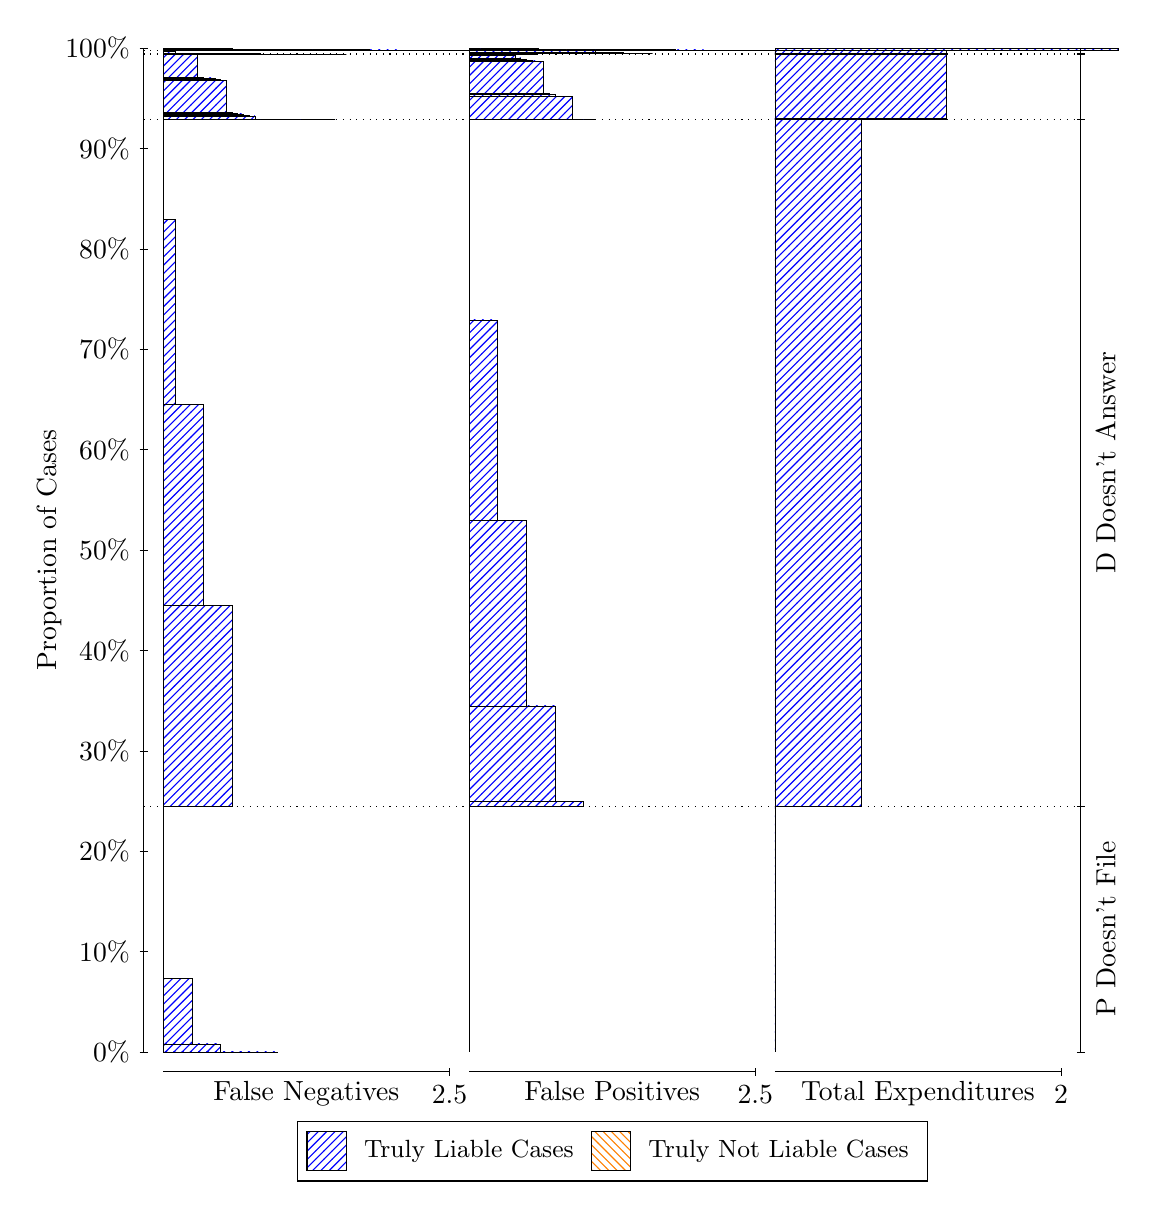
\begin{tikzpicture}
\draw[black, very thin] (1.5,1.75) -- (1.5,14.5);
\node[rotate=90, text=black, anchor=center] at (0.3, 8.125) {Proportion of Cases};
\draw[black, very thin] (1.45,1.75) -- (1.55,1.75);
\node[text=black, anchor=east] at (1.45, 1.75) {0\%};
\draw[black, very thin] (1.45,3.025) -- (1.55,3.025);
\node[text=black, anchor=east] at (1.45, 3.025) {10\%};
\draw[black, very thin] (1.45,4.3) -- (1.55,4.3);
\node[text=black, anchor=east] at (1.45, 4.3) {20\%};
\draw[black, very thin] (1.45,5.575) -- (1.55,5.575);
\node[text=black, anchor=east] at (1.45, 5.575) {30\%};
\draw[black, very thin] (1.45,6.85) -- (1.55,6.85);
\node[text=black, anchor=east] at (1.45, 6.85) {40\%};
\draw[black, very thin] (1.45,8.125) -- (1.55,8.125);
\node[text=black, anchor=east] at (1.45, 8.125) {50\%};
\draw[black, very thin] (1.45,9.4) -- (1.55,9.4);
\node[text=black, anchor=east] at (1.45, 9.4) {60\%};
\draw[black, very thin] (1.45,10.675) -- (1.55,10.675);
\node[text=black, anchor=east] at (1.45, 10.675) {70\%};
\draw[black, very thin] (1.45,11.95) -- (1.55,11.95);
\node[text=black, anchor=east] at (1.45, 11.95) {80\%};
\draw[black, very thin] (1.45,13.225) -- (1.55,13.225);
\node[text=black, anchor=east] at (1.45, 13.225) {90\%};
\draw[black, very thin] (1.45,14.5) -- (1.55,14.5);
\node[text=black, anchor=east] at (1.45, 14.5) {100\%};

\draw[black, very thin] (13.4,1.75) -- (13.4,14.5);
\draw[black, very thin] (13.35,1.75) -- (13.45,1.75);
\node[anchor=west] at (13.35, 1.75) {};
\draw[black, very thin] (13.35,4.8716) -- (13.45,4.8716);
\node[anchor=west] at (13.35, 4.8716) {};
\draw[black, very thin] (13.35,13.596) -- (13.45,13.596);
\node[anchor=west] at (13.35, 13.596) {};
\draw[black, very thin] (13.35,14.415) -- (13.45,14.415);
\node[anchor=west] at (13.35, 14.415) {};
\draw[black, very thin] (13.35,14.434) -- (13.45,14.434);
\node[anchor=west] at (13.35, 14.434) {};
\draw[black, very thin] (13.35,14.47) -- (13.45,14.47);
\node[anchor=west] at (13.35, 14.47) {};
\draw[black, very thin] (13.35,14.5) -- (13.45,14.5);
\node[anchor=west] at (13.35, 14.5) {};

\draw[black, very thin, pattern color=blue, pattern=north east lines] (1.75,1.75) rectangle (3.2033,1.75);
\draw[black, very thin, pattern color=blue, pattern=north east lines] (1.75,1.75) rectangle (2.84,1.7509);
\draw[black, very thin, pattern color=blue, pattern=north east lines] (1.75,1.7509) rectangle (2.4767,1.8532);
\draw[black, very thin, pattern color=blue, pattern=north east lines] (1.75,1.8532) rectangle (2.1133,2.6848);
\draw[black, very thin, pattern color=orange, pattern=north west lines] (1.75,2.6848) rectangle (1.75,2.6848);
\draw[black, very thin, pattern color=blue, pattern=north east lines] (1.75,2.6848) rectangle (1.75,4.8716);
\draw[black, very thin, pattern color=blue, pattern=north east lines] (1.75,4.8716) rectangle (2.622,7.4215);
\draw[black, very thin, pattern color=blue, pattern=north east lines] (1.75,7.4215) rectangle (2.2587,9.9698);
\draw[black, very thin, pattern color=blue, pattern=north east lines] (1.75,9.9698) rectangle (1.8953,12.322);
\draw[black, very thin, pattern color=orange, pattern=north west lines] (1.75,12.322) rectangle (1.75,12.322);
\draw[black, very thin, pattern color=blue, pattern=north east lines] (1.75,12.322) rectangle (1.75,13.596);
\draw[black, very thin, pattern color=blue, pattern=north east lines] (1.75,13.596) rectangle (3.93,13.596);
\draw[black, very thin, pattern color=blue, pattern=north east lines] (1.75,13.596) rectangle (3.7847,13.596);
\draw[black, very thin, pattern color=blue, pattern=north east lines] (1.75,13.596) rectangle (3.6393,13.596);
\draw[black, very thin, pattern color=blue, pattern=north east lines] (1.75,13.596) rectangle (3.5667,13.596);
\draw[black, very thin, pattern color=blue, pattern=north east lines] (1.75,13.596) rectangle (3.494,13.596);
\draw[black, very thin, pattern color=blue, pattern=north east lines] (1.75,13.596) rectangle (3.4213,13.596);
\draw[black, very thin, pattern color=blue, pattern=north east lines] (1.75,13.596) rectangle (3.3487,13.596);
\draw[black, very thin, pattern color=blue, pattern=north east lines] (1.75,13.596) rectangle (3.276,13.596);
\draw[black, very thin, pattern color=blue, pattern=north east lines] (1.75,13.596) rectangle (3.2033,13.596);
\draw[black, very thin, pattern color=blue, pattern=north east lines] (1.75,13.596) rectangle (3.1307,13.596);
\draw[black, very thin, pattern color=blue, pattern=north east lines] (1.75,13.596) rectangle (3.058,13.597);
\draw[black, very thin, pattern color=blue, pattern=north east lines] (1.75,13.597) rectangle (2.9853,13.597);
\draw[black, very thin, pattern color=blue, pattern=north east lines] (1.75,13.597) rectangle (2.9127,13.637);
\draw[black, very thin, pattern color=blue, pattern=north east lines] (1.75,13.637) rectangle (2.84,13.649);
\draw[black, very thin, pattern color=blue, pattern=north east lines] (1.75,13.649) rectangle (2.7673,13.665);
\draw[black, very thin, pattern color=blue, pattern=north east lines] (1.75,13.665) rectangle (2.6947,13.673);
\draw[black, very thin, pattern color=blue, pattern=north east lines] (1.75,13.673) rectangle (2.622,13.682);
\draw[black, very thin, pattern color=blue, pattern=north east lines] (1.75,13.682) rectangle (2.5493,14.089);
\draw[black, very thin, pattern color=blue, pattern=north east lines] (1.75,14.089) rectangle (2.4767,14.104);
\draw[black, very thin, pattern color=blue, pattern=north east lines] (1.75,14.104) rectangle (2.404,14.121);
\draw[black, very thin, pattern color=blue, pattern=north east lines] (1.75,14.121) rectangle (2.3313,14.121);
\draw[black, very thin, pattern color=blue, pattern=north east lines] (1.75,14.121) rectangle (2.2587,14.125);
\draw[black, very thin, pattern color=blue, pattern=north east lines] (1.75,14.125) rectangle (2.186,14.415);
\draw[black, very thin, pattern color=blue, pattern=north east lines] (1.75,14.415) rectangle (2.0407,14.415);
\draw[black, very thin, pattern color=blue, pattern=north east lines] (1.75,14.415) rectangle (1.8953,14.415);
\draw[black, very thin, pattern color=orange, pattern=north west lines] (1.75,14.415) rectangle (1.75,14.415);
\draw[black, very thin, pattern color=blue, pattern=north east lines] (1.75,14.415) rectangle (4.0753,14.415);
\draw[black, very thin, pattern color=blue, pattern=north east lines] (1.75,14.415) rectangle (3.712,14.415);
\draw[black, very thin, pattern color=blue, pattern=north east lines] (1.75,14.415) rectangle (3.3487,14.418);
\draw[black, very thin, pattern color=blue, pattern=north east lines] (1.75,14.418) rectangle (2.9853,14.434);
\draw[black, very thin, pattern color=blue, pattern=north east lines] (1.75,14.434) rectangle (2.622,14.434);
\draw[black, very thin, pattern color=orange, pattern=north west lines] (1.75,14.434) rectangle (1.75,14.434);
\draw[black, very thin, pattern color=blue, pattern=north east lines] (1.75,14.434) rectangle (2.622,14.434);
\draw[black, very thin, pattern color=blue, pattern=north east lines] (1.75,14.434) rectangle (2.2587,14.435);
\draw[black, very thin, pattern color=blue, pattern=north east lines] (1.75,14.435) rectangle (1.8953,14.456);
\draw[black, very thin, pattern color=orange, pattern=north west lines] (1.75,14.456) rectangle (1.75,14.456);
\draw[black, very thin, pattern color=blue, pattern=north east lines] (1.75,14.456) rectangle (1.75,14.47);
\draw[black, very thin, pattern color=blue, pattern=north east lines] (1.75,14.47) rectangle (5.8193,14.47);
\draw[black, very thin, pattern color=blue, pattern=north east lines] (1.75,14.47) rectangle (5.456,14.47);
\draw[black, very thin, pattern color=blue, pattern=north east lines] (1.75,14.47) rectangle (5.0927,14.47);
\draw[black, very thin, pattern color=blue, pattern=north east lines] (1.75,14.47) rectangle (4.7293,14.476);
\draw[black, very thin, pattern color=blue, pattern=north east lines] (1.75,14.476) rectangle (4.366,14.487);
\draw[black, very thin, pattern color=blue, pattern=north east lines] (1.75,14.487) rectangle (4.0027,14.487);
\draw[black, very thin, pattern color=blue, pattern=north east lines] (1.75,14.487) rectangle (3.712,14.487);
\draw[black, very thin, pattern color=blue, pattern=north east lines] (1.75,14.487) rectangle (3.6393,14.487);
\draw[black, very thin, pattern color=blue, pattern=north east lines] (1.75,14.487) rectangle (3.3487,14.487);
\draw[black, very thin, pattern color=blue, pattern=north east lines] (1.75,14.487) rectangle (2.9853,14.487);
\draw[black, very thin, pattern color=blue, pattern=north east lines] (1.75,14.487) rectangle (2.622,14.492);
\draw[black, very thin, pattern color=blue, pattern=north east lines] (1.75,14.492) rectangle (2.2587,14.499);
\draw[black, very thin, pattern color=blue, pattern=north east lines] (1.75,14.499) rectangle (1.8953,14.5);
\draw[black, very thin, pattern color=orange, pattern=north west lines] (1.75,14.5) rectangle (1.75,14.5);
\draw[black, very thin, pattern color=blue, pattern=north east lines] (1.75,14.5) rectangle (1.75,14.5);
\draw[black, very thin, pattern color=orange, pattern=north west lines] (5.6333,1.75) rectangle (5.6333,1.75);
\draw[black, very thin, pattern color=blue, pattern=north east lines] (5.6333,1.75) rectangle (5.6333,4.8716);
\draw[black, very thin, pattern color=orange, pattern=north west lines] (5.6333,4.8716) rectangle (7.0867,4.8716);
\draw[black, very thin, pattern color=blue, pattern=north east lines] (5.6333,4.8716) rectangle (7.0867,4.9278);
\draw[black, very thin, pattern color=blue, pattern=north east lines] (5.6333,4.9278) rectangle (6.7233,6.1455);
\draw[black, very thin, pattern color=blue, pattern=north east lines] (5.6333,6.1455) rectangle (6.36,8.4979);
\draw[black, very thin, pattern color=blue, pattern=north east lines] (5.6333,8.4979) rectangle (5.9967,11.046);
\draw[black, very thin, pattern color=blue, pattern=north east lines] (5.6333,11.046) rectangle (5.6333,13.596);
\draw[black, very thin, pattern color=orange, pattern=north west lines] (5.6333,13.596) rectangle (7.232,13.596);
\draw[black, very thin, pattern color=blue, pattern=north east lines] (5.6333,13.596) rectangle (7.232,13.596);
\draw[black, very thin, pattern color=orange, pattern=north west lines] (5.6333,13.596) rectangle (7.0867,13.596);
\draw[black, very thin, pattern color=blue, pattern=north east lines] (5.6333,13.596) rectangle (7.0867,13.596);
\draw[black, very thin, pattern color=orange, pattern=north west lines] (5.6333,13.596) rectangle (6.9413,13.596);
\draw[black, very thin, pattern color=blue, pattern=north east lines] (5.6333,13.596) rectangle (6.9413,13.886);
\draw[black, very thin, pattern color=blue, pattern=north east lines] (5.6333,13.886) rectangle (6.8687,13.89);
\draw[black, very thin, pattern color=orange, pattern=north west lines] (5.6333,13.89) rectangle (6.796,13.89);
\draw[black, very thin, pattern color=blue, pattern=north east lines] (5.6333,13.89) rectangle (6.796,13.89);
\draw[black, very thin, pattern color=blue, pattern=north east lines] (5.6333,13.89) rectangle (6.7233,13.907);
\draw[black, very thin, pattern color=orange, pattern=north west lines] (5.6333,13.907) rectangle (6.6507,13.907);
\draw[black, very thin, pattern color=blue, pattern=north east lines] (5.6333,13.907) rectangle (6.6507,13.922);
\draw[black, very thin, pattern color=blue, pattern=north east lines] (5.6333,13.922) rectangle (6.578,14.329);
\draw[black, very thin, pattern color=blue, pattern=north east lines] (5.6333,14.329) rectangle (6.5053,14.338);
\draw[black, very thin, pattern color=blue, pattern=north east lines] (5.6333,14.338) rectangle (6.4327,14.346);
\draw[black, very thin, pattern color=blue, pattern=north east lines] (5.6333,14.346) rectangle (6.36,14.362);
\draw[black, very thin, pattern color=blue, pattern=north east lines] (5.6333,14.362) rectangle (6.2873,14.374);
\draw[black, very thin, pattern color=blue, pattern=north east lines] (5.6333,14.374) rectangle (6.2147,14.414);
\draw[black, very thin, pattern color=blue, pattern=north east lines] (5.6333,14.414) rectangle (6.142,14.414);
\draw[black, very thin, pattern color=blue, pattern=north east lines] (5.6333,14.414) rectangle (6.0693,14.415);
\draw[black, very thin, pattern color=blue, pattern=north east lines] (5.6333,14.415) rectangle (5.9967,14.415);
\draw[black, very thin, pattern color=blue, pattern=north east lines] (5.6333,14.415) rectangle (5.924,14.415);
\draw[black, very thin, pattern color=blue, pattern=north east lines] (5.6333,14.415) rectangle (5.8513,14.415);
\draw[black, very thin, pattern color=blue, pattern=north east lines] (5.6333,14.415) rectangle (5.7787,14.415);
\draw[black, very thin, pattern color=blue, pattern=north east lines] (5.6333,14.415) rectangle (5.706,14.415);
\draw[black, very thin, pattern color=blue, pattern=north east lines] (5.6333,14.415) rectangle (5.6333,14.415);
\draw[black, very thin, pattern color=orange, pattern=north west lines] (5.6333,14.415) rectangle (6.5053,14.415);
\draw[black, very thin, pattern color=blue, pattern=north east lines] (5.6333,14.415) rectangle (6.5053,14.415);
\draw[black, very thin, pattern color=blue, pattern=north east lines] (5.6333,14.415) rectangle (6.142,14.432);
\draw[black, very thin, pattern color=blue, pattern=north east lines] (5.6333,14.432) rectangle (5.7787,14.434);
\draw[black, very thin, pattern color=blue, pattern=north east lines] (5.6333,14.434) rectangle (5.6333,14.434);
\draw[black, very thin, pattern color=orange, pattern=north west lines] (5.6333,14.434) rectangle (7.9587,14.434);
\draw[black, very thin, pattern color=blue, pattern=north east lines] (5.6333,14.434) rectangle (7.9587,14.434);
\draw[black, very thin, pattern color=blue, pattern=north east lines] (5.6333,14.434) rectangle (7.5953,14.448);
\draw[black, very thin, pattern color=blue, pattern=north east lines] (5.6333,14.448) rectangle (7.232,14.469);
\draw[black, very thin, pattern color=blue, pattern=north east lines] (5.6333,14.469) rectangle (6.8687,14.47);
\draw[black, very thin, pattern color=blue, pattern=north east lines] (5.6333,14.47) rectangle (6.5053,14.47);
\draw[black, very thin, pattern color=orange, pattern=north west lines] (5.6333,14.47) rectangle (9.7027,14.47);
\draw[black, very thin, pattern color=blue, pattern=north east lines] (5.6333,14.47) rectangle (9.7027,14.47);
\draw[black, very thin, pattern color=orange, pattern=north west lines] (5.6333,14.47) rectangle (9.3393,14.47);
\draw[black, very thin, pattern color=blue, pattern=north east lines] (5.6333,14.47) rectangle (9.3393,14.47);
\draw[black, very thin, pattern color=orange, pattern=north west lines] (5.6333,14.47) rectangle (8.976,14.47);
\draw[black, very thin, pattern color=blue, pattern=north east lines] (5.6333,14.47) rectangle (8.976,14.47);
\draw[black, very thin, pattern color=orange, pattern=north west lines] (5.6333,14.47) rectangle (8.6127,14.47);
\draw[black, very thin, pattern color=blue, pattern=north east lines] (5.6333,14.47) rectangle (8.6127,14.477);
\draw[black, very thin, pattern color=blue, pattern=north east lines] (5.6333,14.477) rectangle (8.2493,14.482);
\draw[black, very thin, pattern color=blue, pattern=north east lines] (5.6333,14.482) rectangle (7.886,14.483);
\draw[black, very thin, pattern color=blue, pattern=north east lines] (5.6333,14.483) rectangle (7.5227,14.483);
\draw[black, very thin, pattern color=orange, pattern=north west lines] (5.6333,14.483) rectangle (7.232,14.483);
\draw[black, very thin, pattern color=blue, pattern=north east lines] (5.6333,14.483) rectangle (7.232,14.483);
\draw[black, very thin, pattern color=blue, pattern=north east lines] (5.6333,14.483) rectangle (7.1593,14.483);
\draw[black, very thin, pattern color=blue, pattern=north east lines] (5.6333,14.483) rectangle (6.8687,14.483);
\draw[black, very thin, pattern color=orange, pattern=north west lines] (5.6333,14.483) rectangle (6.8687,14.483);
\draw[black, very thin, pattern color=blue, pattern=north east lines] (5.6333,14.483) rectangle (6.8687,14.483);
\draw[black, very thin, pattern color=blue, pattern=north east lines] (5.6333,14.483) rectangle (6.5053,14.483);
\draw[black, very thin, pattern color=orange, pattern=north west lines] (5.6333,14.483) rectangle (6.5053,14.483);
\draw[black, very thin, pattern color=blue, pattern=north east lines] (5.6333,14.483) rectangle (6.5053,14.493);
\draw[black, very thin, pattern color=blue, pattern=north east lines] (5.6333,14.493) rectangle (6.142,14.493);
\draw[black, very thin, pattern color=blue, pattern=north east lines] (5.6333,14.493) rectangle (6.142,14.5);
\draw[black, very thin, pattern color=blue, pattern=north east lines] (5.6333,14.5) rectangle (5.7787,14.5);
\draw[black, very thin, pattern color=blue, pattern=north east lines] (5.6333,14.5) rectangle (5.7787,14.5);
\draw[black, very thin, pattern color=blue, pattern=north east lines] (5.6333,14.5) rectangle (5.6333,14.5);
\draw[black, very thin, pattern color=orange, pattern=north west lines] (9.5167,1.75) rectangle (9.5167,1.75);
\draw[black, very thin, pattern color=blue, pattern=north east lines] (9.5167,1.75) rectangle (9.5167,4.8716);
\draw[black, very thin, pattern color=orange, pattern=north west lines] (9.5167,4.8716) rectangle (10.607,4.8716);
\draw[black, very thin, pattern color=blue, pattern=north east lines] (9.5167,4.8716) rectangle (10.607,13.596);
\draw[black, very thin, pattern color=orange, pattern=north west lines] (9.5167,13.596) rectangle (11.697,13.596);
\draw[black, very thin, pattern color=blue, pattern=north east lines] (9.5167,13.596) rectangle (11.697,13.609);
\draw[black, very thin, pattern color=orange, pattern=north west lines] (9.5167,13.609) rectangle (11.697,13.609);
\draw[black, very thin, pattern color=blue, pattern=north east lines] (9.5167,13.609) rectangle (11.697,14.415);
\draw[black, very thin, pattern color=orange, pattern=north west lines] (9.5167,14.415) rectangle (11.697,14.415);
\draw[black, very thin, pattern color=blue, pattern=north east lines] (9.5167,14.415) rectangle (11.697,14.434);
\draw[black, very thin, pattern color=orange, pattern=north west lines] (9.5167,14.434) rectangle (11.697,14.434);
\draw[black, very thin, pattern color=blue, pattern=north east lines] (9.5167,14.434) rectangle (11.697,14.47);
\draw[black, very thin, pattern color=orange, pattern=north west lines] (9.5167,14.47) rectangle (13.877,14.47);
\draw[black, very thin, pattern color=blue, pattern=north east lines] (9.5167,14.47) rectangle (13.877,14.5);
\draw[black, dotted] (1.5,4.8716) -- (13.4,4.8716);
\draw[black, dotted] (1.5,13.596) -- (13.4,13.596);
\draw[black, dotted] (1.5,14.415) -- (13.4,14.415);
\draw[black, dotted] (1.5,14.434) -- (13.4,14.434);
\draw[black, dotted] (1.5,14.47) -- (13.4,14.47);
\draw[black, very thin] (1.75,1.5) -- (5.3833,1.5);
\node[text=black, anchor=north] at (3.5667, 1.5) {False Negatives};
\draw[black, very thin] (5.3833,1.45) -- (5.3833,1.55);
\node[text=black, anchor=north] at (5.3833, 1.45) {2.5};

\draw[black, very thin] (5.6333,1.5) -- (9.2667,1.5);
\node[text=black, anchor=north] at (7.45, 1.5) {False Positives};
\draw[black, very thin] (9.2667,1.45) -- (9.2667,1.55);
\node[text=black, anchor=north] at (9.2667, 1.45) {2.5};

\draw[black, very thin] (9.5167,1.5) -- (13.15,1.5);
\node[text=black, anchor=north] at (11.333, 1.5) {Total Expenditures};
\draw[black, very thin] (13.15,1.45) -- (13.15,1.55);
\node[text=black, anchor=north] at (13.15, 1.45) {2};

\node[text=black, centered, rotate=90] at (13.72, 3.3108) {P Doesn't File};
\node[text=black, centered, rotate=90] at (13.72, 9.2339) {D Doesn't Answer};





\draw (7.449999999999999,1.5) node[draw=none] (baseCoordinate) {};
\begin{scope}[align=center]
        \matrix[scale=0.5, draw=black, below=0.5cm of baseCoordinate, nodes={draw}, column sep=0.1cm]{
            \node[rectangle, draw, minimum width=0.5cm, minimum height=0.5cm, pattern color=blue, pattern=north east lines] {}; &
            \node[draw=none, font=\small, text=black] (B) {Truly Liable Cases}; &
            \node[rectangle, draw, minimum width=0.5cm, minimum height=0.5cm, pattern color=orange, pattern=north west lines] {}; &
            \node[draw=none, font=\small, text=black] (B) {Truly Not Liable Cases}; \\
            };
\end{scope}

\end{tikzpicture}
\end{document}